\chapter{Ejercicios de diseño}


 \section{Sistemas fotovoltaicos de conexión a red}


 \subsection{Entorno del diseño}

Ante la implantación de un nuevo hipermercado en A Coruña ($\phi=43.37\degree\mathrm{\, N}$),
el equipo de arquitectos e ingenieros al cargo del diseño toman en
consideración las implicaciones del documento HE5 del Código Técnico
de la Edificación. Consideran que la ubicación del correspondiente
generador fotovoltaico se debe realizar en la cubierta del centro.
En esta cubierta, a pesar de los elementos ya proyectados, no hay
problemas de espacio ni sombras que afecten al generador. No obstante,
por criterios estéticos deciden alinear el generador con la fachada
principal del edificio. Este centro tendrá una superficie construida
de $\SI{8500}{\meter\squared}$, con una fachada desviada $15\degree$
del Sur. 
\begin{enumerate}
\item ¿Cuales son los ángulos óptimos de inclinación y orientación de este
sistema? Con las limitaciones que impone el edificio, ¿qué orientación
e inclinación se deben adoptar? ¿Es posible cumplir las especificaciones
de pérdidas por orientación e inclinación que marca el documento HE5
del CTE?
\item Como primera aproximación, y suponiendo un módulo con una eficiencia
del 13\%, ¿qué área aproximada de la cubierta ocupará el generador
fotovoltaico?
\item Como resultado de una primera búsqueda de mercado, los cálculos iniciales
se realizarán con un módulo y un inversor con las siguientes características.
¿Qué configuración de generador e inversores propone utilizar?

\begin{minipage}[t]{0.4\columnwidth}%
Módulo:
\begin{itemize}
\item $P_{mpp}=\SI{175}{\Wp}$
\item $V_{mpp}=\SI{35.4}{\volt}$
\item $I_{mpp}=\SI{4.9}{\ampere}$
\item $I_{sc}=\SI{5.45}{\ampere}$
\item $V_{oc}=\SI{43.6}{\volt}$
\item 72 células en serie.
\end{itemize}
%
\end{minipage}%
\hspace{0.4cm}
\begin{minipage}[t]{0.4\columnwidth}%
Inversor:
\begin{itemize}
\item $P_{nom}=\SI{2.5}{\kW}$
\item Ventana MPP={[}125-450{]} Vdc
\item $V_{max}=\SI{450}{Vdc}$
\end{itemize}
%
\end{minipage}

\item Está previsto que el consumo eléctrico del hipermercado sea de $\SI{200}{\kWh\per\meter\squared}$.
¿Qué proporción de esta energía consumida representa la producción
del generador fotovoltaico?
\end{enumerate}

\subsubsection{Solución}

\begin{enumerate}
\item Los ángulos óptimos son:\[
\beta_{opt}=3.7+0.69\cdot\phi=33.37\degree\]
\[
\alpha_{opt}=0^{\circ}\]
Dado que se ha optado por alinear el generador con el edificio, la
orientación del generador debera ser de $\alpha=15\degree$. Dado
que el generador se instalará en la cubierta, como una instalacion
estática convencional, la inclinación puede ser elegida sin restricciones.
Así, elegimos el número entero más próximo: $\beta=35\degree$.\\
Las pérdidas debidas a orientación e inclinación, según la fórmula
propuesta en el HE5-CTE son, con los ángulos escogidos, de 0.84\%.
Este valor es inferior a las exigencias del CTE, independientemente
de la modalidad de integración.
\item La potencia que exige el HE5-CTE para este edificio es $P_{g}^{*}=\SI{12.8}{\kilo\Wp}$.
Utilizamos la definición de eficiencia de un generador fotovoltaico:\[
\eta=0.13=\frac{P_{g}^{*}}{A\cdot\SI{1000}{\watt\per\meter\squared}}\rightarrow A=\SI{98.5}{\meter\squared}\]
Si utilizamos ROT=2 (estática), el área de cubierta que necesitamos
es de aproximadamente $\SI{200}{\meter\squared}$.
\item Para una temperatura ambiente de $25\celsius$ (ecuación \ref{eq:Vmpp_inv})
obtenemos $V_{mpp}=\SI{30.6}{\volt}$. Para el límite inferior de
la ventana MPP del inversor obtenemos $125/30.6=4.1$, mientras que
el límite superior obtenemos $450/30.6=14.7$. \\
Para adecuar el generador a la tensión máxima del inversor hay
que corregir la tensión de circuito abierto del módulo para las condiciones
de radiación y temperatura de la ecuación \ref{eq:Voc_inv}:\begin{eqnarray*}
T_{c} & = & -10+200\cdot\frac{47-20}{800}=\SI{-3.25}{\celsius}\\
V_{oc} & = & 43.6-2.3\cdot10^{-3}\cdot72\cdot(-3.25-25)=\SI{48.28}{\volt}\end{eqnarray*}
Por tanto, el número máximo de módulos en serie es $450/48.28=9.32$.
Se deberá elegir un número comprendido entre 5 y 9. \\
Si se opta por $N_{s}=8$ y $N_{p}=2$ la potencia equivalente
es $\SI{2800}{\Wp}$ por cada inversor, lo que supone un factor
de $1.12$ sobre la potencia del inversor, valor aceptable para una
instalación estática. Si se opta por $N_{s}=7$ y $N_{p}=2$ la potencia
es ahora $\SI{2450}{\Wp}$ por cada inversor, lo que supone
una potencia algo inferior a la nominal del inversor. Sin embargo,
la combinación de estas dos configuraciones permite alcanzar una potencia
total de $\SI{12950}{\Wp}$ con 3 inversores de 7 módulos en
serie y 2 inversores de 8 módulos en serie. Si los 5 inversores utilizan
series de 8 módulos, la potencia total será $\SI{13650}{\Wp}$.
La elección final depende de varios factores, como ya ha sido relatado
en el capítulo correspondiente.
\item Supongamos que se dispone de información de la radiación en el plano
horizontal en la localidad. Para estimar la radiación efectiva en
el plano del generador debe recorrerse el itinerario detallado en el texto, bien sea por los propios
medios o recurriendo a algún software de cálculo. Como ejemplo, recurrimos
a la información disponible en el mapa de la figura \ref{fig:GefFixed}
la productividad de este sistema es, aproximadamente, $Y_{f}=\SI{1000}{\kWh\per\kilo\Wp}$.
Suponiendo una potencia instalada igual a la calculada en el punto
2, el sistema fotovoltaico aporta menos del 1\% del consumo eléctrico
del edificio.

\end{enumerate}

\clearpage{}

\subsection{Entorno del diseño}

Para promover el uso de sistemas fotovoltaicos en los centros
educativos del municipio, el Ayuntamiento de Coslada ha abierto un
concurso para la instalación de sistemas fotovoltaicos conectados a
red.

Para facilitar la evaluación de las ofertas el pliego de condiciones
técnicas del concurso fija unos determinados parámetros del diseño:
\begin{itemize}
\item El ángulo de inclinación del generador debe ser de $30\degree$
  con orientación Sur. La latitud del lugar es, para los efectos del
  cálculo, igual a $41\degree$.
\item Cada centro contará con un sistema fotovoltaico con una potencia
  de generador de $\SI{15}{\kilo\Wp}$.
\item Cada sistema debe contar con dos o más inversores funcionando en
  paralelo.
\item El generador se ubicará en la cubierta plana de los centros. Las
  sombras por objetos externos al generador son despreciables a los
  efectos del cálculo.
\item La radiación global anual en el plano horizontal en el municipio
  es de $\SI{1740}{\kilo\Wh\per\meter\squared}$.
\end{itemize}

En base a estas condiciones debe responder a las siguientes
cuestiones:

\begin{enumerate}
\item En el contexto del Código Técnico de la Edificación, y de
  acuerdo a la fórmula recogida en su documento HE5, ¿qué pérdidas por
  orientación e inclinación suponen los ángulos exigidos en el pliego
  de condiciones del concurso?

  Clasificando este sistema como ``general'' dentro de las tipologías
  de integración arquitectónica, ¿son permisibles estos valores según
  el documento HE5?
\item Proponga una configuración eléctrica de generador fotovoltaico e
  inversores para cumplir los requisitos del pliego con el módulo
  YL-200%
\footnote{Información disponible en
  \url{http://yinglisolar.com/uploadfiles/product/1264589110_SUQ0Z2rCJS.pdf}}
 y con la gama de inversores SMC 4600A%
\footnote{Información
   disponible en \url{http://www.sma-iberica.com/es/productos/inversores-solares/sunny-mini-central/sunny-mini-central-4600a-5000a-6000a.html}}.
\item Organizando el generador en varias hileras de una única altura
  de módulos en vertical, ¿qué distancia entre hileras permite obtener
  cuatro horas libres de sol durante el solsticio de invierno?
\item ¿Qué esquema de tierra debe emplear? En caso de necesitar algún
  tipo de conexión a tierra, ¿qué relación tendrá con el sistema de
  tierras del centro escolar?
\item Con un \emph{performance ratio} de $0.75$ y un factor de sombras
  de $0.02$, calcule la \textbf{productividad} del sistema
  fotovoltaico.
\end{enumerate}

\subsubsection{Solución}

\begin{enumerate}
\item Utilizamos la ecuación correspondiente con los datos del
  enunciado, $100\cdot[1.2\cdot10^{-4}\cdot(30-41+10)^{2}+3.5 \cdot 10^{-5} \cdot
  0^{2}]$, para obtener un valor de $0.012$. Por tanto, las pérdidas debidas a
  la orientación e inclinación son despreciables y, evidentemente,
  encajan sin problemas con los requisitos del CTE-HE5.
\item En primer lugar calculamos la temperatura para la tensión máxima
  admisible:
  \[
  T_c=-10+200 \cdot \frac{46-20}{800}=\SI{-3.5}{\celsius}
  \]
  La tensión de circuito abierto correspondiente es:
  \[
  V_{oc}=33.3-0.0037 \cdot 33 \cdot (-3.5-25)=\SI{36.81}{\volt}
  \]
  Así, el número máximo de módulos en serie es:
  \[
  N_{sMAX}=\frac{600}{36.81}=16.3
  \]
  y, por tanto, $N_{sMAX}=16$.

  Hacemos lo propio para la ventana MPP.
  \[
  T_c=25+1000 \cdot \frac{46-20}{800}=\SI{57.5}{\celsius}
  \]
  La tensión de circuito abierto correspondiente es:
  \[
  V_{oc}=33.3-0.0037 \cdot 33 \cdot (57.5-25)=\SI{29.3}{\volt}
  \]
  Utilizando la aproximación de factor de forma constante tenemos:
  \[
  V_{mpp}=V_{oc} \cdot \frac{V_{mpp}^*}{V_{oc}^*}=\SI{23.14}{\volt}
  \]

  Así, el número de módulos en serie correspondiente al límite
  superior de la ventana MPP es:
  \[
  N_{sMPP}^{max}=\frac{480}{23.14}=20.74
  \]
  y, por tanto, $N_{sMPP}^{max}=20$.

  El número de módulos en serie correspondiente al límite inferior de
  la ventana MPP es:
  \[
  N_{sMPP}^{max}=\frac{246}{23.14}=10.6
  \]
  y, por tanto, $N_{sMPP}^{min}=11$.

  En resumen, $11 \leq N_s \leq 16$.

  Para el cálculo de ramas en paralelo basta con realizar la siguiente
  operación:
  \[
  N_{pMAX}=\frac{I_{max,INV}}{I_{scM}}=\frac{26}{8.22}=3.16
  \]

  Por tanto, $N_{pMAX}=3$.

  Una posible configuración consiste en utilizar tres inversores SMC
  4600A, cada uno de ellos alimentado por un generador fotovoltaico de
  $\SI{5200}{\Wp}$, compuesto por 2 ramas de 13 módulos en
  serie. Esta configuración supone un generador de
  $\SI{15.6}{\kilo\Wp}$ con una potencia de inversor de
  $\SI{14.8}{\kilo\watt}$ ($P_{g}^{*}/P_{inv}=1.13$).

\item La distancia entre filas (calculada entre inicio de la posterior
  y fin de la anterior) es:
  \[
  d=\frac{h}{\tan(61-41)}=\frac{1.495 \cdot
    \sin(30)}{\tan(20)}=\SI{2.05}{\meter}
  \]

  Para calcular la distancia entre puntos equivalentes (entre inicio e
  inicio de filas, por ejemplo) hay que tener en cuenta la proyección
  de cada fila: $1.495 \cdot \cos(41)=\SI{1.294}{\meter}$. Así, el ROT
  equivalente es $ROT=\frac{2.05+1.294}{1.495}=2.23$.

\item En la zona del generador fotovoltaico (DC) el esquema adecuado
  es IT, mientras que en la zona comprendida entre inversor y red (AC)
  el esquema debe ser TT. La conexión a tierra de las masas del
  sistema se llevará a cabo empleando la puesta a tierra existente en
  el edificio.

\item A partir de la radiación global anual en el plano horizontal
  calculamos la incidente en la orientación óptima:
  \[
  \frac{G_{a}(0)}{G_{a}(\beta_{opt})}=1-4.46\cdot10^{-4}\cdot 31.99 -
  1.19\cdot10^{-4}\cdot 31.99^{2}=0.864
  \]
  y a continuación la irradiación efectiva incidente en el plano del
  generador:
  \[
  \frac{G_{efa}(\beta,\alpha)}{G_{a}(\beta_{opt})} = -1.218 \cdot
  10^{-4} \cdot (1.99)^{2} + 2.892 \cdot 10^{-4} \cdot (1.99) + 0.9314
  = 0.9315
  \]

  De esta forma $G_{ef,a}=\frac{0.9315}{0.864} \cdot 1740 =
  \SI{1875}{\kilo\Wh\per\meter\squared}$, y la productividad del
  sistema es
  \[Y_f = 1875 \cdot 0.75 \cdot (1-0.02) =
  \SI{1378.8}{\kilo\Wh\per\kilo\Wp}\].


\end{enumerate}

\clearpage{}


\subsection{Entorno del diseño}

Un antiguo aeródromo localizado cerca del pueblo leonés de Rodrigatos
de la Obispalía ($\phi=42.3\degree\mathrm{N}$), abandonado durante
más de 50 años, es ahora recibido como herencia por un conjunto de
tres hermanos. Sus variadas orientaciones profesionales e ideológicas
confluyen en la decisión común de emplear este espacio para alojar
una instalación fotovoltaica de conexión a red. El dinero y propiedades
que, junto con el aeródromo, conforman el conjunto de la herencia,
les permite proyectar un sistema fotovoltaico de una potencia del
orden de 1 MWp.

Dado su escaso conocimiento técnico sobre la tecnología fotovoltaica
deciden requerir los servicios de una consultoría especializada, siendo
usted su persona de contacto. En este contexto, le solicitan su respuesta
sobre los siguientes aspectos:
\begin{enumerate}
\item ¿Cuales son los ángulos óptimos de inclinación y orientación de este
sistema? ¿Qué angulos propone emplear?
\item Como resultado de una primera búsqueda de mercado, los cálculos iniciales
se realizarán con un módulo y un inversor con las siguientes
características:

%
\begin{minipage}[t]{0.4\columnwidth}%
Módulo:
\begin{itemize}
\item $P_{mpp}^{*}=\SI{165}{\Wp}$
\item $V_{mpp}^{*}=\SI{34.3}{\volt}$
\item $I_{mpp}^{*}=\SI{4.8}{\ampere}$
\item $I_{sc}^{*}=\SI{5.4}{\ampere}$
\item $V_{oc}^{*}=\SI{43.7}{\volt}$
\item 72 células en serie.
\item $TONC=\SI{47}{\celsius}$
\item $\frac{dV_{oc}}{dT_{c}}=\SI{-0.36}{\percent\per\kelvin}$
\item Dimensiones: $\SI{1593}{\milli\metre}\times\SI{790}{\milli\metre}$
\end{itemize}
%
\end{minipage}%
\hspace{0.5cm}
\begin{minipage}[t]{0.4\columnwidth}%
Inversor:
\begin{itemize}
\item $P_{nom}=\SI{100}{\kW}$
\item Ventana MPP={[}405-750{]} Vdc
\item $V_{max}=\SI{900}{V_{dc}}$
\item $I_{max}=\SI{286}{\ampere}$
\end{itemize}
%
\end{minipage}

\begin{enumerate}
\item ¿Qué área aproximada deberá tener el terreno para un sistema estático,
un sistema de seguimiento a doble eje y un sistema de eje horizontal
norte-sur? 
\item ¿Qué configuración de generador e inversores propone utilizar?
\end{enumerate}
\item Sobre la base de un generador fotovoltaico estático de 1015 kWp (independientemente
del resultado del apartado anterior) orientado al Sur e inclinado
$30\degree$ (independientemente del resultado del primer apartado),
estime la energía anual producida por el sistema. Suponga que el rendimiento
global del sistema es del 73\%. Las posibles sombras arrojadas por
los arboles del perimetro de la finca pueden cuantificarse en un 3\%
de pérdidas. Según una estación meteorológica cercana, la irradiación
global anual en el plano horizontal es de $\SI{1680}{\kWh\per\meter\squared}$. 
\end{enumerate}

\subsubsection{Solución}
\begin{enumerate}
\item Los ángulos óptimos son $\beta_{opt}=3.7+0.69\cdot\left|\phi\right|=32.9\degree$
y $\alpha_{opt}=0^{\circ}$. Es razonable emplear $\beta=30\degree$
y $\alpha=0\degree$.
\item En primer lugar hacemos una estimación del área ocupada sin tener
en cuenta la configuración eléctrica.

\begin{enumerate}
\item Utilizamos la definición de eficiencia de un dispositivo fotovoltaico
y la información del módulo recogida en la ficha técnica:\[
\eta=\frac{P_{m}^{*}}{A_{m}\cdot\SI{1000}{\watt\per\meter\squared}}=\frac{165}{(1.59\cdot0.79)\cdot1000}=13.1\%\]
Un generador de $\SI{1000}{\kilo\Wp}$ compuesto con este módulo
ocupa un área de \[
A_{g}=\frac{\SI{1000}{\kilo\Wp}}{0.131\cdot\SI{1}{\kilo\watt\per\meter\squared}}=\SI{7627.1}{\meter\squared}\]
Para un sistema estático (ROT=2) el área de terreno que necesitamos
es de: \[
A_{T}=\SI{15254.2}{\meter\squared}\]
Para un sistema de seguimiento con eje horizontal Norte-Sur (ROT=4)
el área de terreno que necesitamos es de: \[
A_{T}=\SI{30508.4}{\meter\squared}\]
Para un sistema de doble eje (ROT=6) el área de terreno que necesitamos
es de: \[
A_{T}=\SI{45762.6}{\meter\squared}\]

\item Con el inversor elegido configuramos el generador fotovoltaico en
diez conjuntos. En primer lugar elegimos el número de módulos en serie.
\[
N_{sMAX}=\frac{V_{MAX,inv}}{V_{ocm}(G=\SI{200}{\watt\per\meter\squared},\, T_{a}=\SI{-10}{\celsius})}\]
La temperatura de trabajo es: \[
T_{c}=-10+200\cdot\frac{47-20}{800}=\SI{-3.25}{\celsius}\]
y, por tanto (teniendo en cuenta la información de la relación de
la tensión con la temperatura del módulo), \[
V_{ocm}=43.7-\frac{\Delta V_{oc}}{\Delta T_{c}}\Delta T_{c}=43.7-(0.36\%\cdot43.7)\cdot(-3.25-25)=\SI{48.14}{\volt}\]
De esta forma\[
N_{s,MAX}=\frac{900}{48.14}=18.7\rightarrow N_{s,MAX}=18\]
A continuación, comparamos la tensión del punto de máxima potencia
con la ventana del inversor. Ahora la temperatura de trabajo es:\[
T_{c}=25+1000\cdot\frac{47-20}{800}=\SI{58.75}{\celsius}\]
y la tensión en circuito abierto es:\[
V_{ocm}=\SI{38.4}{\volt}\]
Suponiendo constante el factor de forma con la temperatura:\[
V_{mpp}=\frac{V_{mpp}^{*}}{V_{oc}^{*}}\cdot38.4=\SI{30.14}{\volt}\]
De esta forma \[
N_{sMPP}^{max}=\frac{750}{30.14}=24.9\rightarrow N_{sMPP}^{max}=24\]
y\[
N_{sMPP}^{min}=\frac{405}{30.14}=13.44\rightarrow N_{sMPP}^{min}=14\]
De esta forma, la ventana de elección es $N_{s}\in\left[14,18\right]$.
Realicemos ahora los cálculos para el número de ramas en paralelo:
\[
N_{p,MAX}=\frac{I_{MAX,inv}}{I_{scm}^{*}}=\frac{286}{5.4}=52.96\rightarrow N_{p,MAX}=52\]
Como se ha explicado en la sección \ref{sub:ConfiguracionGenerador},
la configuración del generador se elige teniendo en cuenta varios
factores de forma que no existe una solución única. Por ejemplo, para
esta combinación de módulo e inversor, una posible configuración es
utilizar $N_{p}=46$ y $N_{s}=14$ por inversor. Así obtenemos un
generador compuesto por un total de 6440 módulos, lo que implica una
potencia total de generador de $\SI{1062}{\kilo\Wp}$.
\item En primer lugar hay que calcular la irradiación global efectiva en
el plano del generador. Utilizamos la relación entre la irradiación
en el plano horizontal y en el plano óptimo:\[
\frac{G_{a}(0)}{G_{a}(\beta_{opt})}=1-4.46\cdot10^{-4}\cdot32.9-1.19\cdot10^{-4}\cdot32.9^{2}=0.856\]
y por tanto\[
G_{a}(\beta_{opt})=1680/0.856=\SI{1962.6}{\kWh\per\meter\squared}\]
Con este resultado podemos obtener la irradiación efectiva:\[
\frac{G_{efa}(\beta,\alpha)}{G_{a}(\beta_{opt})}=-1.218\cdot10^{-4}(30-32.9)^{2}+2.892\cdot10^{-4}\cdot(30-32.9)+0.9314=0.9295\]
luego\[
G_{efa}(\beta,\alpha)=0.9295\cdot1962.6=\SI{1824.3}{\kWh\per\meter\squared}\]
La energía anual producida por el sistema es:\[
E_{ac}=1015\cdot1824.3\cdot0.73\cdot(1-0.03)=\SI{1311.1}{\mega\Wh}\]

\end{enumerate}
\end{enumerate}

\clearpage{}

\section{Sistemas Fotovoltaicos Autónomos}

\subsection{Entorno del diseño}

En el contexto de un programa de electrificación rural en la región
brasileña cercana a Posse (Goiás) (latitud promedio $\phi=14.1\degree\mathrm{S}$)
se acomete la implantación de sistemas fotovoltaicos para centros
comunales. De acuerdo con los datos de campo obtenidos se propone
un equipamiento de consumo promedio, valido para la mayoría de estos
centros de esta región. Ante la falta de mayor información se asume
que el consumo será constante durante todo el año, según las cifras
recogidas en las siguientes tablas\footnote{Cada equipo se emplea durante un
tiempo determinado por sus horas de uso a una potencia constante; para
la nevera, como es habitual, se señala la energía diaria consumida.}:

\begin{flushleft}
%
\begin{minipage}[t]{0.5\columnwidth}%
Cargas DC

\begin{flushleft}
\begin{tabular}{>{\raggedright}p{1.5cm}>{\centering}p{1.5cm}>{\centering}p{1.5cm}>{\centering}p{1cm}}
\toprule 
Nombre & Unidades & Potencia (W) & Horas Uso\tabularnewline
\midrule 
Luminaria & 5 & 15 & 4\tabularnewline
\midrule 
Radio & 1 & 50 & 2\tabularnewline
\midrule 
Nevera & 1 & \multicolumn{2}{c}{$\SI{300}{\Wh}$}\tabularnewline
\midrule 
Ventilador & 2 & 50 & 4\tabularnewline
\bottomrule
\end{tabular}
\par\end{flushleft}%
\end{minipage}%
\begin{minipage}[t]{0.5\columnwidth}%
Cargas AC

\begin{flushleft}
\begin{tabular}{>{\centering}p{1.5cm}>{\centering}p{1.5cm}>{\centering}p{1.5cm}>{\centering}p{1cm}}
\toprule 
Nombre & Unidades & Potencia (W)  & Horas Uso\tabularnewline
\midrule 
Ordenador PC & 1 & 200 & 4\tabularnewline
\bottomrule
\end{tabular}
\par\end{flushleft}%
\end{minipage}
\par\end{flushleft}
\begin{enumerate}
\item ¿Cuales son los ángulos óptimos de inclinación y orientación de este
sistema? 
\item Proponga sendos valores para las capacidades de generación ($C_{A}$)
y de acumulación ($C_{s}$).
\item Se opta por una tensión de trabajo de $\SI{24}{\volt}$. Suponiendo
que el módulo a suministrar tiene una tensión nominal de 12 V y una
corriente nominal de 2 A, ¿qué configuración de generador propone? 
\item Para limitar el envejecimiento de los acumuladores, el programa propone
una profundidad máxima de descarga del 60\%. Del catálogo de baterías
puede seleccionar elementos de tensión nominal $\SI{12}{\volt}$,
y capacidades de 180, 200, 240 y 300 Ah. ¿Qué capacidad de vaso utilizará
y cuál será la configuración de la batería? Según la información del
programa de electrificación, la radiación diaria incidente en el generador
en esta zona para el mes peor es $G_{d,m}(I)=\SI{5}{\kilo\Wh\per\meter\squared}$. 
\end{enumerate}

\subsubsection{Solución}

\begin{enumerate}
\item Dado que la aplicación debe garantizar el suministro durante el mes
peor, la inclinación debe ser\[
\beta_{opt}=|\phi|+10^{\circ}=25.1^{\circ}\]
La orientación, como de costumbre, debe ser:\[
\alpha_{opt}=0^{\circ}\]
pero, dado que la instalación se ubica en el hemisferio Sur, quedará
dirigida hacia el horizonte Norte. Para la inclinación, elegimos un
$\beta=25\degree$.
\item Según las recomendaciones de diversos estudios y normativas, para
este tipo de consumo de electrificación rural, es razonable usar $C_{A}=1.1$
y $C_{S}=5$.

\item Utilizando las ecuaciones correspondientes obtenemos
los siguientes resultados:\[
L_{T}=\SI{2046.8}{\Wh}\]
\[
L=\SI{2534.7}{\Wh}\]
y, teniendo en cuenta la tensión del sistema, resulta:\[
Q_{L}=\SI{105.6}{\amperehour}\]
Por tanto, el generador debe tener una corriente de:\[
I_{G}^{*}=\SI{23.2}{\ampere}\]
A partir de los valores del módulo suministrados en el enunciado,
configuramos el generador:\[
N_{S}=24/12=2\]
\[
N_{p}=23.2/2=11.6\rightarrow N_{p}=12\]
Comprobamos que al traducir el valor de $I_{G}^{*}$ al número de
paneles, teniendo en cuenta los valores discretos de tensión y corriente,
obtenemos un tamaño de generador superior al que resulta del primer
cálculo. Por tanto, no es necesario añadir un factor adicional para
tener en cuenta las pérdidas por temperatura.
\item De la ecuación correspondiente obtenemos:\[
C_{U}=\SI{528.1}{\amperehour}\]
y por tanto, teniendo en cuenta la profundidad de descarga, la capacidad
de la batería necesaria es:\[
C_{B}=528.1/0.6=\SI{880.1}{\amperehour}\]
Por tanto, necesitaremos 3 baterías de $\SI{300}{\amperehour}$ conectadas
en paralelo. Por otra parte, debido a la tensión de las baterías disponibles
será necesario conectar dos elementos en serie para conseguir que
el sistema funcione a $\SI{24}{\volt}$. Así, se deberán emplear 6
baterías de $\SI{300}{\amperehour}$ conectando 3 ramas en paralelo
de 2 baterías en serie.\\
Es necesario resaltar que las conexiones en paralelo de baterías
debe ser evitada en la medida de lo posible para evitar la degradación
acelerada de los elementos. Sin embargo, en este caso la disponibilidad
de baterías no permite otra opción. 
\end{enumerate}

\clearpage{}


\subsection{Entorno del diseño}

El Banco Interamericano de Desarrollo ha puesto en marcha una
licitación internacional para el suministro de sistemas fotovoltaicos
de electrificación rural en determinados municipios del Altiplano
Boliviano, situados en una latitud de $15\degree\mathrm{S}$.

Esta licitación incluye tres sistemas diferenciados:
\begin{itemize}
\item \textbf{Sistemas domiciliares}, cuyo consumo consta de 2
  lámparas fluorescentes de $\SI{15}{\watt}$ cada una y una radio de
  $\SI{50}{\watt}$. Se estima que el uso de las lámparas es de 6 horas
  diarias, y el de la radio de 1 hora diaria. La tensión nominal del
  sistema es de $\SI{12}{\volt}$.
\item \textbf{Sistemas comunales}, cuyo consumo consta de 5 lámparas
  fluorescentes de $\SI{15}{\watt}$ cada una, una radio de
  $\SI{50}{\watt}$ y una televisión B-N (DC) de $\SI{300}{\watt}$. La
  iluminación está activa durante 4 horas al día, y la radio y
  televisión durante 2 horas al día. La tensión nominal del sistema es
  de $\SI{24}{\volt}$.
\item \textbf{Postas de salud}, cuyo consumo consta de 6 lámparas
  fluorescentes de $\SI{15}{\watt}$ cada una y una nevera para vacunas
  con un consumo diario de $\SI{300}{\Wh}$. La iluminación se
  emplea durante 6 horas al día. La tensión nominal del sistema es de
  $\SI{24}{\volt}$.
\end{itemize}

Según el pliego, el generador fotovoltaico debe estar inclinado a
$15\degree$.

Elija los valores adecuados de $C_A$ y $C_S$ para cada tipología y
dimensione el generador fotovoltaico y sistema de acumulación,
empleando el módulo KC65T%
\footnote{Información disponible en
  \url{http://www.kyocerasolar.com/assets/001/5170.pdf}.} 
y la gama PowerSafe OPzS%
\footnote{Información disponible en \url{http://www.enersys-emea.com/reserve/pdf/EN-OPzS-RS-005_0111.pdf}}. Al dimensionar, especifique que
configuración eléctrica de generador y sistema de acumulación es
necesario utilizar en cada tipología.

Para poder emplear los datos recogidos en la ficha técnica de la
batería, puede suponer que la capacidad en $C_{100}$ es un
aproximadamente $1.35 \cdot C_{10}$. La profundidad de descarga debe
ser $PD=0.7$.

Considere que los rendimientos característicos del sistema son
$\eta_{r}=0.95$, $\eta_{bat}=0.85$ y $\eta_{c}=0.98$.

Según los datos de la NASA-SSE recogidos en el pliego de licitación,
las medias mensuales de radiación global diaria incidente en un plano
inclinado $15\degree$ son ($\si{\kilo\Wh\per\meter\squared}$):

\begin{tabular}[center]{cccccccccccc}
  \toprule
  Ene & Feb & Mar & Abr & May & Jun & Jul & Ago & Sep & Oct & Nov &
  Dic\\
  \midrule
  4.92 & 4.69 & 4.77 & 4.96 & 4.65 & 4.83 & 5.31 & 5.26 & 5.25 & 5.31 &
  5.29 & 5.06\\
  \bottomrule
\end{tabular}


\subsubsection{Solución}


Según los datos del enunciado, el consumo correspondiente a cada
tipología es (incluyendo la eficiencia del regulador):
\begin{itemize}
\item SHS: $L_T=\SI{242.1}{\Wh}$
\item Centros comunales: $L_T=\SI{1052.6}{\Wh}$
\item Postas de salud: $L_T=\SI{884.2}{\Wh}$
\end{itemize}

Dado que todos los consumos son en corriente continua, teniendo en
cuenta los valores de rendimiento del regulador, la batería y el
cableado, el consumo de diseño es:
\begin{itemize}
\item SHS: $L=\SI{290.6}{\Wh}$
\item Centros comunales: $L=\SI{1263.6}{\Wh}$
\item Postas de salud: $L=\SI{1061.5}{\Wh}$
\end{itemize}
y por tanto, teniendo en cuenta la tensión nominal de cada sistema:

\begin{itemize}
\item SHS: $Q_L=\SI{24.22}{\ampere\hour}$
\item Centros comunales: $Q_L=\SI{52.6}{\ampere\hour}$
\item Postas de salud: $Q_L=\SI{44.3}{\ampere\hour}$
\end{itemize}

Para estas aplicaciones, los valores recomendados de $C_A$ y $C_S$
son:

\begin{itemize}
\item SHS: $C_A=1.1$, $C_s=3$.
\item Centros comunales: $C_A=1.1$, $C_s=5$.
\item Postas de salud: $C_A=1.1$, $C_s=5$.
\end{itemize}

A partir de estos valores se puede realizar el dimensionado de cada
tipología. Todos los cálculos se realizan con el valor de radiación
del mes peor, aquel con menor valor de radiación dado que el consumo
se considera constante:

\begin{itemize}
\item SHS: Con un módulo en serie se alcanza la tensión nominal de
  esta tipología. Para calcular el número de paneles en paralelo
  calculamos la corriente del generador:
  \[
  I_g^* = \frac{1.1 \cdot 24.2}{4.65}=\SI{5.73}{\ampere}
  \]

  Se necesitan 2 módulos en paralelo para conseguir este valor de
  corriente. Por tanto, $N_s=1$ y $N_p=2$.

  Para conseguir la tensión nominal del sistema, con las baterías del
  catálogo suministrado es necesario utilizar 6 vasos en
  serie. Además,
  \[
  C_U=C_s \cdot Q_L = 3 \cdot 24.22 = \SI{72.7}{\ampere\hour}
  \]
  y, por tanto, $C_B= \SI{103.8}{\ampere\hour}$. Cualquier batería del
  catálogo cumple ampliamente este valor. Bastaría con 6 vasos en
  serie de la 4OPZs200. Sería recomendable recurrir a otra gama de
  baterías más adaptada al consumo de esta aplicación.

\item Centro comunal: Con dos módulos en serie se alcanza la tensión
  nominal de esta tipología. Para calcular el número de paneles en
  paralelo calculamos la corriente del generador:
  \[
  I_g^* = \frac{1.1 \cdot 52.6}{4.65}=\SI{12.5}{\ampere}
  \]

  Se necesitan 5 módulos en paralelo para conseguir este valor de
  corriente. Por tanto, $N_s=2$ y $N_p=5$.

  Para conseguir la tensión nominal del sistema, con las baterías del
  catálogo suministrado es necesario utilizar 12 vasos en
  serie. Además,
  \[
  C_U=C_s \cdot Q_L = 5 \cdot 52.6 = \SI{263.3}{\ampere\hour}
  \]
  y, por tanto, $C_B= \SI{376.1}{\ampere\hour}$. La batería 6OPZs300
  cumple este requerimiento (teniendo en cuenta la relación entre
  $C_{10}$ y $C_{100}$). Por tanto, el sistema de acumulación estará
  compuesto por 12 vasos en serie del modelo 6OPZs300.

\item Posta de salud: Con dos módulos en serie se alcanza la tensión
  nominal de esta tipología. Para calcular el número de paneles en
  paralelo calculamos la corriente del generador:
  \[
  I_g^* = \frac{1.1 \cdot 44.3 }{4.65}=\SI{10.5}{\ampere}
  \]

  Se necesitan 3 módulos en paralelo para conseguir este valor de
  corriente. Por tanto, $N_s=2$ y $N_p=3$.

  Para conseguir la tensión nominal del sistema, con las baterías del
  catálogo suministrado es necesario utilizar 12 vasos en
  serie. Además,
  \[
  C_U=C_s \cdot Q_L = 5 \cdot 44.3 = \SI{221.1}{\ampere\hour}
  \]
  y, por tanto, $C_B= \SI{315.9}{\ampere\hour}$. La batería 5OPZs250
  cumple este requerimiento (teniendo en cuenta la relación entre
  $C_{10}$ y $C_{100}$). Por tanto, el sistema de acumulación estará
  compuesto por 12 vasos en serie del modelo 5OPZs250.

\end{itemize}


\subsection{Entorno del diseño}
Se desea alimentar con un sistema fotovoltaico un radioenlace remoto con un consumo constante a una
potencia de $\SI{1}{\kilo\watt}$. Utilizando el método de LLP, proponga
valores de $C_{A}^{'}$ y $C_s$ para obtener un valor de $LLP=10^{-2}$. 

Para reducir el valor de LLP sin aumentar excesivamente el coste del
sistema de generación, se propone incorporar un grupo electrógeno de
$\SI{10}{\kilo\volt\ampere}$. Este equipo proporciona un factor de potencia de
$0.7$ con un consumo de $\SI{0.3}{\litre\per\kilo\Wh}$. Calcule
las horas de funcionamiento y el consumo anual de combustible que será 
necesario para reducir a cero la probabilidad de pérdida de carga.
\subsubsection{Solución}
Las ecuaciones necesarias son:

\begin{align*}
  C_{A}^{'} & = f\cdot C_{S}^{-u} \\
  f &= f_1 + f_2 \cdot \log(\mathrm{LLP}) \\
  u &= \exp(u_1+u_2 \cdot \mathrm{LLP})
\end{align*}

con  $f_1=-0.2169$, $f_2=-0.7865$, $u_1=-1.2138$ y $u_2=-15.280$
(valores para Madrid).

Un valor razonable para la capacidad de acumulación es
$C_s=5$. Empleando las ecuaciones anteriores obtenemos $C_{A}^{'}=0.9$
para el requisito de $LLP=0.01$\footnote{Recordemos que $C_{A}^{'}$ está
relacionado con la capacidad del generador $C_A$  a través de la ecuación:
\begin{equation*}
C_{A}^{'}=C_{A}\cdot\frac{\overline{G_{d}}(0)}{\overline{G_{d}}(\beta,\alpha)}
\end{equation*}
}.

Con este valor de LLP, en términos anuales, el sistema fotovoltaico no será capaz de
suministrar:
\begin{equation}
  \SI{1}{\kilo\watt} \cdot 10^{-2} \cdot 24 \cdot 365 = \SI{87.6}{\kilo\Wh}
\end{equation}

El grupo electrógeno entrega $\SI{10}{\kilo\volt\ampere} \cdot 0.7 =
\SI{7}{\kilo\watt}$ de potencia activa.
Para suministrar toda la energía que el sistema fotovoltaico no es
capaz, el grupo deberá estar en funcionamiento aproximadamente 12.5
horas al año, y consumirá $0.3 \cdot 87.6=\SI{26.3}{\litre}$ al año.

\clearpage{}

\section{Sistemas Fotovoltaicos de Bombeo}


\subsection{Entorno del diseño}


En un lugar situado en la latitud $40^{\circ}\mathrm{S}$, se pretende
llevar a cabo un sistema de bombeo solar directo para abastecer de
agua a una comunidad rural compuesta por 600 personas. Según las medidas
tomadas, la media anual del consumo diario por habitante es de 50
litros. En esta comunidad existe un pozo con una profundidad de 90
metros. Este pozo ha sido sometido a ensayo por la autoridad local,
obteniendo un valor de 30 metros para la altura estática, 50 metros
para la altura dinámica y un caudal máximo de extracción de 10 litros
por segundo. Esta comunidad ha decidido anticiparse a la implantación
del sistema y la construido una casa para albergar los equipos y proteger
el pozo, y asimismo ha levantado un depósito en las cercanías. La
altura de la boca de entrada a este depósito se encuentra a 10 metros
sobre el suelo.
\begin{enumerate}
\item ¿Cuales son los ángulos óptimos de inclinación y orientación de este
sistema? 
\item Calcule la altura total equivalente ($H_{TE}$) despreciando las pérdidas
por fricción en las tuberías. 
\item Sabiendo que en esta localidad la media mensual de la radiación diaria
incidente en el plano del generador durante el mes de diseño es de
$\SI{5}{\kWh\per\meter\squared}$, determine un valor aproximado
de la potencia de generador necesaria. 
\item Si elegimos una bomba de 380 Vac, y un módulo de las siguientes características,
¿qué configuración de generador fotovoltaico propone?\\
 %
\begin{minipage}[t]{1\columnwidth}%
Módulo:
\begin{itemize}
\item $P_{mpp}=\SI{150}{\Wp}$
\item $V_{mpp}=\SI{34.6}{\volt}$
\item $I_{mpp}=\SI{4.35}{\ampere}$
\item $I_{sc}=\SI{4.7}{\ampere}$
\item $V_{oc}=\SI{43.2}{\volt}$
\item 72 células en serie.
\end{itemize}
%
\end{minipage}
\item El depósito construido por la comunidad tiene una capacidad aproximada
de $\SI{50}{\meter\cubed}$. ¿Le parece adecuado? 
\end{enumerate}

\subsubsection{Solución}

\begin{enumerate}
\item En un sistema de bombeo, la inclinación se elige para maximizar
  la producción durante la época de mayor demanda de agua. Por
  tanto, \[ \beta=|\phi|-10^{\circ}=30^{\circ}\]
  \[
  \alpha=0^{\circ}\] Dado que la instalación se ubica en el hemisferio
  Sur, quedará dirigida hacia el horizonte Norte. Estos dos ángulos
  son adecuados para ser implementados en una estructura convencional.
\item Utilizamos la expresión de $H_{TE}$, calculando cada
  sumando:\begin{eqnarray*}
    H_{ot} & = & \SI{10}{\meter}\\
    H_{st} & = & \SI{30}{\meter}\\
    H_{dt} & = & \SI{50}{\meter}\\
    (\frac{H_{dt}-H_{st}}{Q_{max}}) & = & \frac{\SI{20}{\meter}}{\SI{10}{\liter\per\second}}=\SI{0.56}{\hour\per\meter\squared}\\
    Q_{ap} & = &
    0.047\cdot30=\SI{1.41}{\meter\cubed\per\hour}\end{eqnarray*} y por
  tanto:\[ H_{te}=10+30+0.56\cdot1.41+0=\SI{40.8}{\meter}\]

\item Utilizamos la fórmula que aproxima la potencia del generador
  fotovoltaico:\[ P_{g}^{*}=10\cdot\frac{H_{te}\cdot
    Q_{d}}{G_{d}/G*}=10\cdot\frac{40.8\cdot30}{5/1}=\SI{2447}{\Wp}\]
  A partir de esta estimación primera, podemos ajustar el valor de
  potencia necesaria consultando la documentación de un fabricante de
  bombas.  Si recurrimos, por ejemplo, a la documentación de Grundfos,
  teniendo en cuenta la radiación disponible y el caudal requerido,
  elegiremos una bomba del tipo SP5AXX ($30/5=6$, y el número más
  cercano de la gama SP de Grundfos es el 5). Dentro del tipo SP5AXX
  deberemos probar el funcionamiento según el número de etapas de cada
  bomba. En general, varias bombas pueden ser adecuadas desde este
  enfoque de caudal suministrado.  Por ejemplo, la bomba SP5A12 (ver
  nomograma)% en la figura \ref{fig:NomogramaSolucion})
  puede ser una buena solución para esta combinación de altura, caudal
  y radiación. Con este nomograma llegamos a una potencia de generador
  de $\SI{2300}{\Wp}$, valor muy cercano a la primera
  estimación.
  \\
%
  \begin{center}
    % \begin{figure}
    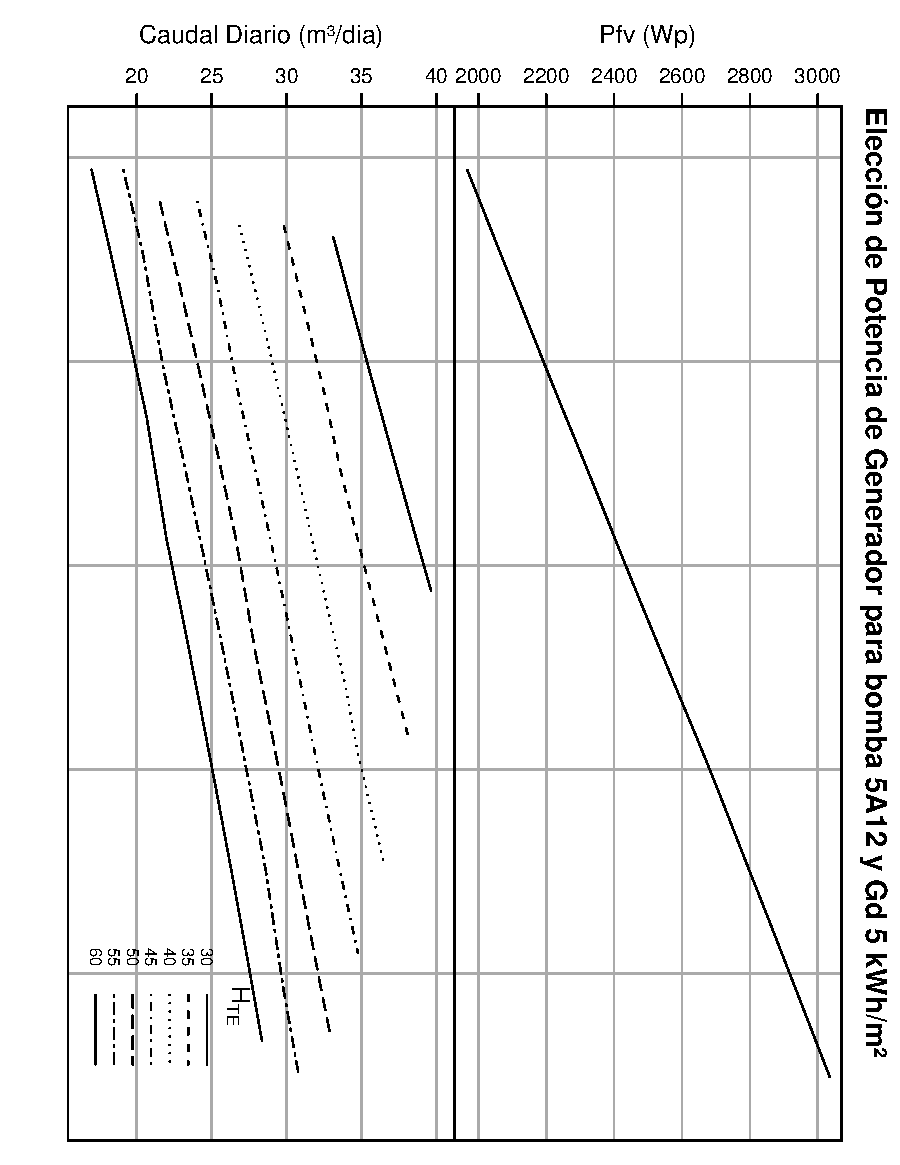
\includegraphics[scale=0.7,
    angle=90]{../figs/AbacoBomba_5Etapas12}

    % \caption{Nomograma para bomba
    % SP5A12\label{fig:NomogramaSolucion}}

    % \end{figure}
  \end{center}

\item Para una bomba que funciona a 380 Vac, deberemos utilizar un
  generador cuya tensión de trabajo sea\[
  V_{dc}=\frac{\sqrt{2}\cdot380}{1.1}=\SI{488.6}{\volt}\] Dado que el
  módulo descrito en el enunciado tiene 72 células en serie, su
  tensión MPP afectada por la temperatura será, aproximadamente de
  $\SI{30}{\volt}$ (recordando que un módulo de 36 células entrega
  $\SI{15}{\volt}$ en funcionamiento real). Por tanto, se deberán
  conectar 17 módulos en serie ($488.6/30=16.3$). Antes de dar por
  buena esta configuración, se debería comprobar que la tensión en
  circuito abierto
  del generador no supera la máxima admisible por el variador. \\
  Esta configuración eléctrica implica una potencia de generador de
  $P_{g}^{*}=17\cdot150=\SI{2550}{\Wp}$, valor algo superior al
  requerido para satisfacer el caudal y vencer la altura manométrica.
  Es frecuente que la potencia resultante de la configuración
  eléctrica del generador para acoplarse al variador sea muy superior
  a la necesaria.  En estos casos se deberá recalcular la
  configuración con módulos de diferente tensión y potencia.
\item $\SI{50}{\meter\cubed}$ es aproximadamente 2 veces el caudal
  diario requerido. Es un tamaño adecuado.
\end{enumerate}


\clearpage{}

\section{Seguridad eléctrica}

\subsection{Entorno del diseño}

Suponiendo que en una planta con varios inversores trifásicos existe
la posibilidad de ubicar los inversores debajo del generador FV (\emph{distribución
en alterna}) o en un centro específico junto al punto de conexión
a red (\emph{distribución en continua}), ¿cuál es la tensión de trabajo
en continua que permite optar por una distribución en continua?. Para
simplificar la resolución esta cuestión se emplearán las siguientes
suposiciones:
\begin{itemize}
\item El inversor trabaja con una eficiencia constante de $0.95$.
\item El inversor no genera potencia reactiva.
\item La caída de tensión admisible es $\Delta V=1.5\%\cdot V_{nom}$, siendo
$V_{nom}$ la tensión de trabajo en cada una de las dos opciones.
Para trifásica, sea $V_{nom}=\SI{400}{\volt}$.
\end{itemize}

\subsubsection{Solución}

El punto crítico que decide sobre el tipo de distribución a emplear
es aquel en el que la masa de cableado coincide en las dos opciones.
Dado que en trifásica se emplean 3 cables (en general, los inversores
fotovoltaicos no exigen el cableado del neutro) y 2 en monofásica,
esta condición es $2\cdot S_{dc}l=3\cdot S_{3ac}l$, donde $l$ es
la longitud de cable a emplear en cuaquiera de las dos opciones. La
sección de la distribución en continua se calcula con:

\[
S_{dc}=\frac{2\cdot l\cdot I_{dc}}{\gamma_\theta\cdot\Delta V_{dc}}\]
mientras que la correspondiente a una distribución trifásica se calcula
con:

\[
S_{3ac}=\frac{\sqrt{3}\cdot l\cdot I_{3ac}}{\gamma_\theta\cdot\Delta V_{3ac}}\]
donde se supone que el factor de potencia del inversor es la unidad.

Estas expresiones pueden reescribirse utilizando la relación entre
potencia, tensión y corriente:

\[
S_{dc}=\frac{2\cdot l\cdot P_{dc}}{\gamma_\theta\cdot1.5\%\cdot V_{dc}^{2}}\]


\[
S_{3ac}=\frac{l\cdot P_{ac}}{\gamma_\theta\cdot1.5\%\cdot V_{ac}^{2}}\]


Con estas ecuaciones la condición primera se expresa de la siguiente
forma:

\[
2\cdot\frac{2\cdot l\cdot P_{dc}}{\gamma_\theta\cdot1.5\%\cdot V_{dc}^{2}}=3\cdot\frac{l\cdot P_{ac}}{\gamma_\theta\cdot1.5\%\cdot V_{ac}^{2}}\]
y teniendo en cuenta las suposiciones propuestas se puede simplificar
para obtener la siguiente relación:\[
\frac{4}{V_{dc}^{2}}=\frac{3\cdot0.95}{400^{2}}\]
que se resuelve con el resultado final: \[
V_{dc}\simeq\SI{473}{\volt}\]


Por tanto, si la configuración del generador fotovoltaico es de tal
forma que su tensión $V_{mpp}$ promedio es igual o superior a $\SI{473}{\volt}$,
la distribución en continua es preferible a la distribución en alterna
desde el punto de vista de masa de conductor necesario.


\clearpage{}

\subsection{Entorno del diseño}\label{EjercicioCableado}
Una planta de seguimiento a dos ejes está compuesta por conjuntos de 4
seguidores conectados a un inversor. Cada uno de los seguidores
soporta un generador fotovoltaico de $\SI{26.4}{\kilo\Wp}$
conformado en 12 ramas de 11 módulos en serie. Las características de
los módulos empleados son:

\begin{itemize}
\item $P_{mpp}=\SI{200}{\Wp}$
\item $V_{mpp}=\SI{46.08}{\volt}$
\item $I_{mpp}=\SI{4.35}{\ampere}$
\item $I_{sc}=\SI{4.7}{\ampere}$
\item $V_{oc}=\SI{57.6}{\volt}$
\end{itemize}


Las separaciones entre seguidores son $L_{ns}=\SI{30}{\metre}$ y
$L_{eo}=\SI{40}{\metre}$. A la salida de cada conjunto de cuatro
seguidores, situado a 1 metro del seguidor más cercano, 
se emplea un cuadro de paralelos que desemboca en un
inversor, tal y como se representa en el esquema siguiente.

\begin{center}
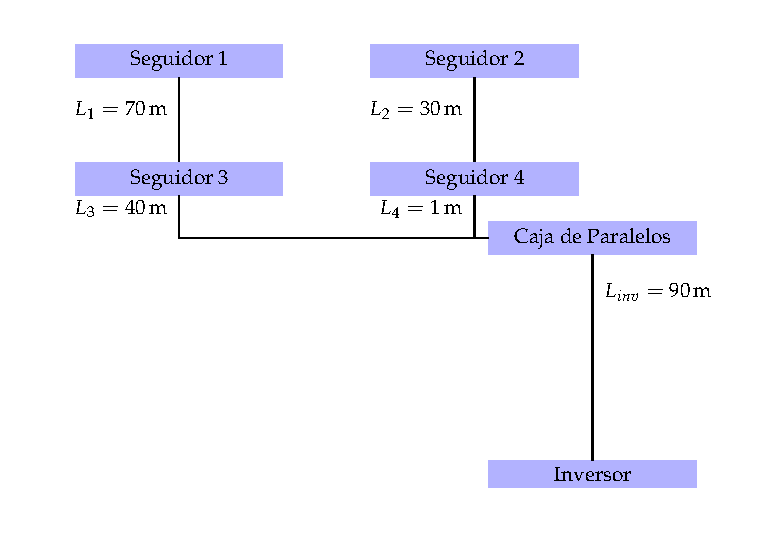
\includegraphics{../figs/EjercicioUbicacionSeguidores}  
\end{center}


Elija secciones adecuadas para los cables que conectan cada seguidor del
primer grupo con la caja de paralelos número 1, y para los cables que
conectan esta caja con el inversor.

\subsubsection{Solución}

Suponemos que el conductor es cobre y el aislamiento es polietileno
reticulado (XLPE). La distribución será en corriente continua con
cables unipolares enterrados.

En primer lugar aplicamos el criterio de caída de tensión con la fórmula:

\[S_{dc} =  \frac{2\cdot l_{dc}\cdot I_{dc}}{\gamma_\theta\cdot\Delta V_{dc}}\]

Según el apartado 5 de la ITC-BT-40, la caída de tensión será inferior
al $1.5\%$ de la tensión nominal. Dado que existen dos tramos (desde el
seguidor hasta la caja de paralelos, y desde la caja hasta el
inversor), esta condición implica que la suma de las dos caídas de
tensión no supere el límite establecido. De esta forma, existe un
grado de libertad (dos incógnitas con una única condición) que sólo
puede resolverse formalmente optimizando el coste de cable total. 

Para evitar la complejidad de este ejercicio de
optimización\footnote{La referencia \cite{Perpinan2012b} detalla el
  procedimiento de cálculo que permite optimizar la masa de cable.}, imponemos una
caída de tensión razonable en cada tramo y resolvemos el valor de
sección correspondiente. Por ejemplo, imponemos una caída de tensión
de $0.5\%$ en el primer tramo y de $1\%$  en el segundo.

Así, para el primer tramo los cálculos se basan en las siguientes condiciones:

\begin{align*}
  I & = 12 \cdot 4.35 = \SI{52.2}{\ampere}\\
  V_{nom} & = 11 \cdot 46.08 = \SI{506.88}{\volt}\\
  \Delta V & = \SI{2.53}{\volt}
\end{align*}

y los resultados son:

\begin{align*}
  s_1 & = \SI{51.49}{\milli\meter\squared}\\
  s_2 & = \SI{22.07}{\milli\meter\squared}\\
  s_3 & = \SI{29.41}{\milli\meter\squared}\\
  s_4 & = \SI{0.74}{\milli\meter\squared}\\
\end{align*}

A continuación, debemos comprobar que estas secciones cumplen el
criterio térmico. En las condiciones detalladas al comienzo de esta
solución, en la ITC-BT-07 comprobamos que la temperatura máxima en
servicio permanente para un cable con aislamiento XLPE es de
$\SI{90}{\celsius}$ (tabla 2). 

Al tratarse de conductor cobre e instalación enterrada, para averiguar
la intensidad máxima admisible por cada una de las secciones
calculadas, empleamos la primera columna (XLPE) de la primera
mitad (terna de cables unipolares) de la tabla 5. Esta tabla supone
que la temperatura del terreno es de $\SI{25}{\celsius}$, que los
cables están a una profundidad de $\SI{0.7}{\meter}$ y que el terreno
tiene una resistividad térmica de $\SI{1}{\kelvin\meter\per\watt}$.

Si la temperatura del terreno es diferente hay que utilizar la tabla 6
(que muestra que a mayor temperatura menor corriente máxima
admisible). Si el terreno tiene una resistividad térmica diferente
corregimos con la tabla 7 (que muestra que a mayor resistividad del
terreno menor corriente máxima admisible). Si la profundidad de
enterramiento es diferente las correcciones están recogidas en la
tabla 9 (donde a mayor profundidad menor corriente máxima
admisible). Además, si la conducción se realiza bajo tubo, hay que
corregir con un factor de $0.8$.

Por otra parte, al ser distribución en continua, la conducción no es
en ternas sino en conjuntos de \emph{dos} cables
unipolares. Corregimos con un factor de $1.225$. Además, en el tramo
comprendido entre los seguidores 3 y 4, y entre la caja de paralelos y
el inversor, los pares de cables conviven con otras agrupaciones. En
este caso hay que emplear la tabla 8 para reducir convenientemente la
corriente máxima admisible con un factor de 0.8.

Según el apartado 5 de la ITC-BT-40, el cable debe ser dimensionado
para una intensidad no inferior al $125\%$ de la máxima intensidad del
generador. Esta máxima intensidad se corresponde con la corriente de
cortocircuito. Así, para el primer tramo la corriente de referencia es
$\SI{70.5}{\ampere}$.  Tomando como buenas las
condiciones para las que está elaborada la tabla 5, y corrigiendo con
un factor de $1.225$ (par de cables en lugar de terna) y otro de $0.8$
(agrupaciones de cables en una misma zanja), esta corriente de
referencia obliga a emplear, al menos, una sección de
$\SI{10}{\milli\meter\squared}$. 

Por tanto, las secciones a utilizar en este primer tramo son:

\begin{align*}
  s_1 & = \SI{70}{\milli\meter\squared}\\
  s_2 & = \SI{25}{\milli\meter\squared}\\
  s_3 & = \SI{35}{\milli\meter\squared}\\
  s_4 & = \SI{10}{\milli\meter\squared}\\
\end{align*}

Para el segundo tramo (entre caja de paralelos e inversor), las
condiciones son:

\begin{align*}
  I & =\SI{208.8}{\ampere}\\
  V_{nom} & = \SI{506.88}{\volt}\\
  \Delta V & = \SI{5.07}{\volt}\\
  L & = \SI{90}{\meter}
\end{align*}

que conducen a una sección de $s=\SI{132.5}{\milli\meter\squared}$,
que corresponde a una sección normalizada de
$\SI{150}{\milli\meter\squared}$.

En este segundo tramo, con las mismas consideraciones anteriores, 
la corriente de referencia para el criterio
térmico es $\SI{282}{\ampere}$, valor que obliga a emplear, al menos,
una sección de $\SI{95}{\milli\meter\squared}$. Así, el valor obtenido
es adecuado.

La figura siguiente resume los resultados obtenidos.

\begin{center}
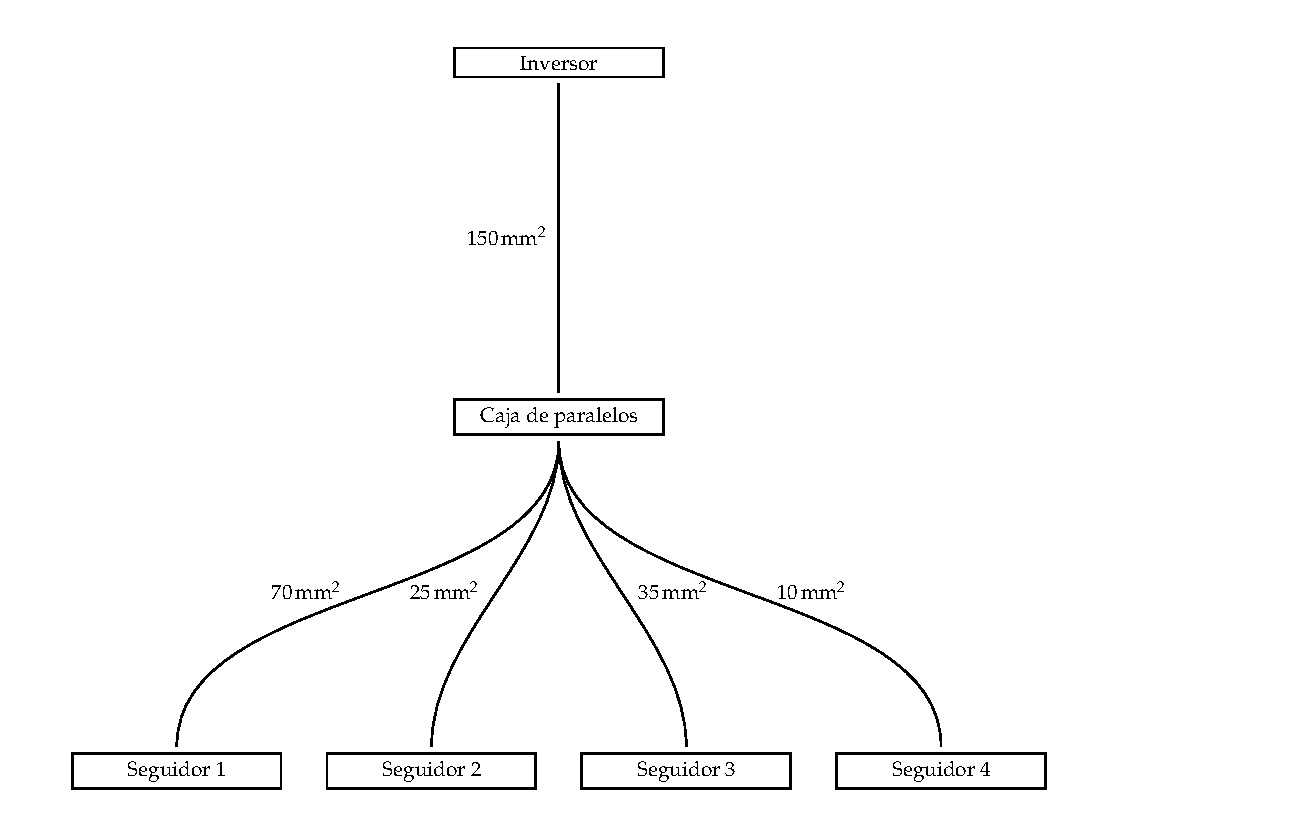
\includegraphics{../figs/Cableado}  
\end{center}


%%% Local Variables:
%%% mode: LaTex
%%% TeX-master: "ESF.tex"
%%% End: 